\begin{frame}{Quality of Generated Protein w.r.t. Length}%ProLLaMA vs. ESM2 (Baseline) Model}
%\begin{center}
\begin{columns}
	\begin{column}{0.5\textwidth}
		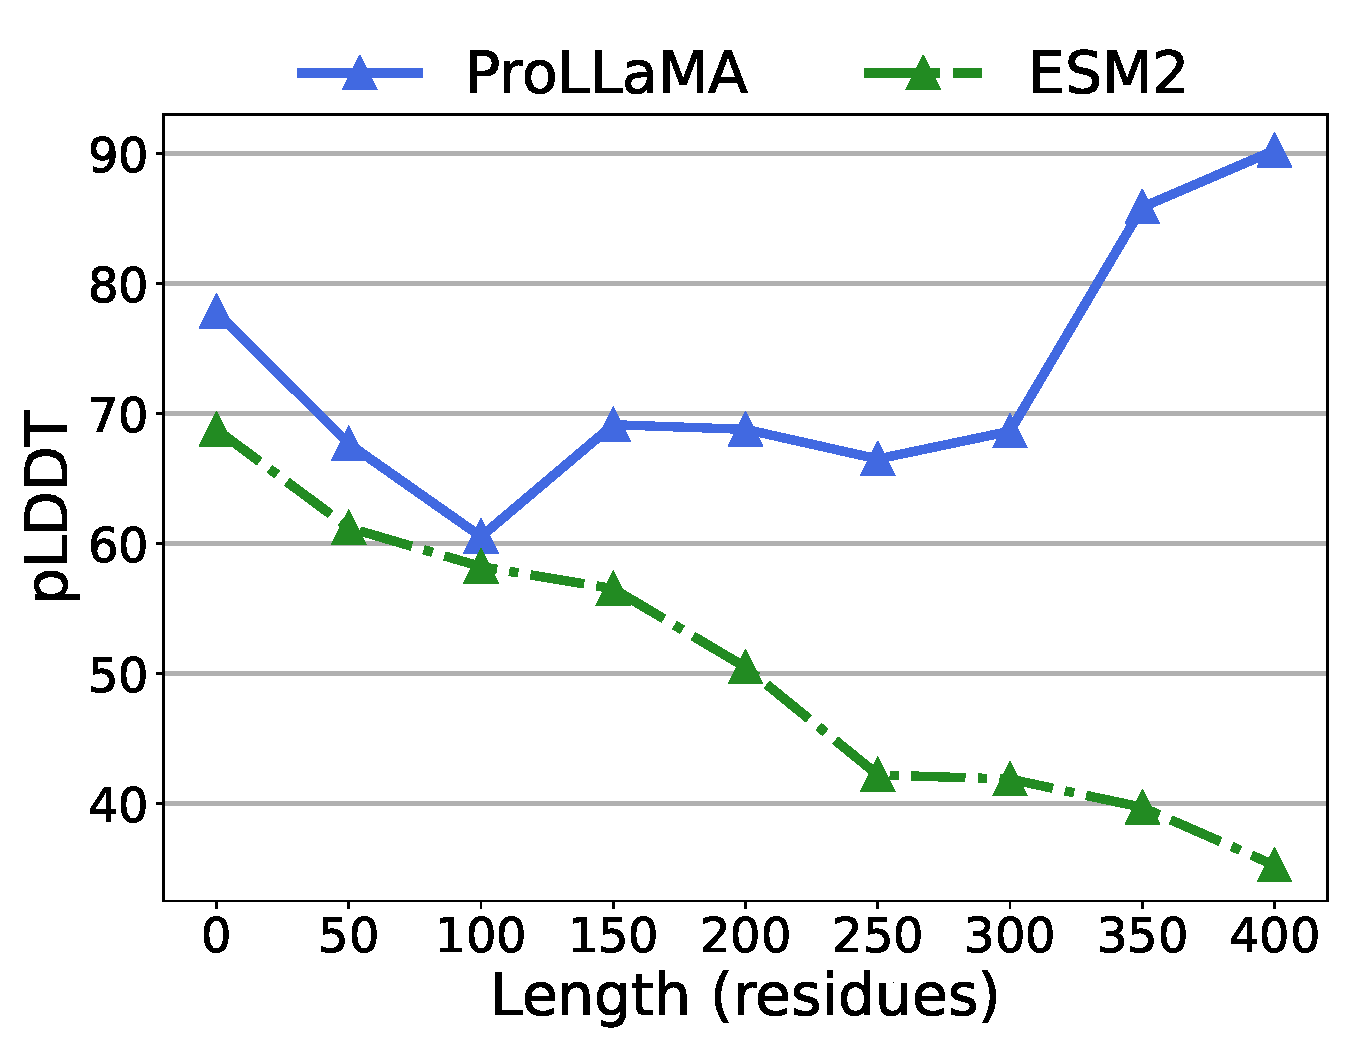
\includegraphics[scale=0.23]{images/combined_length_plddt_zhexiantu.pdf}
		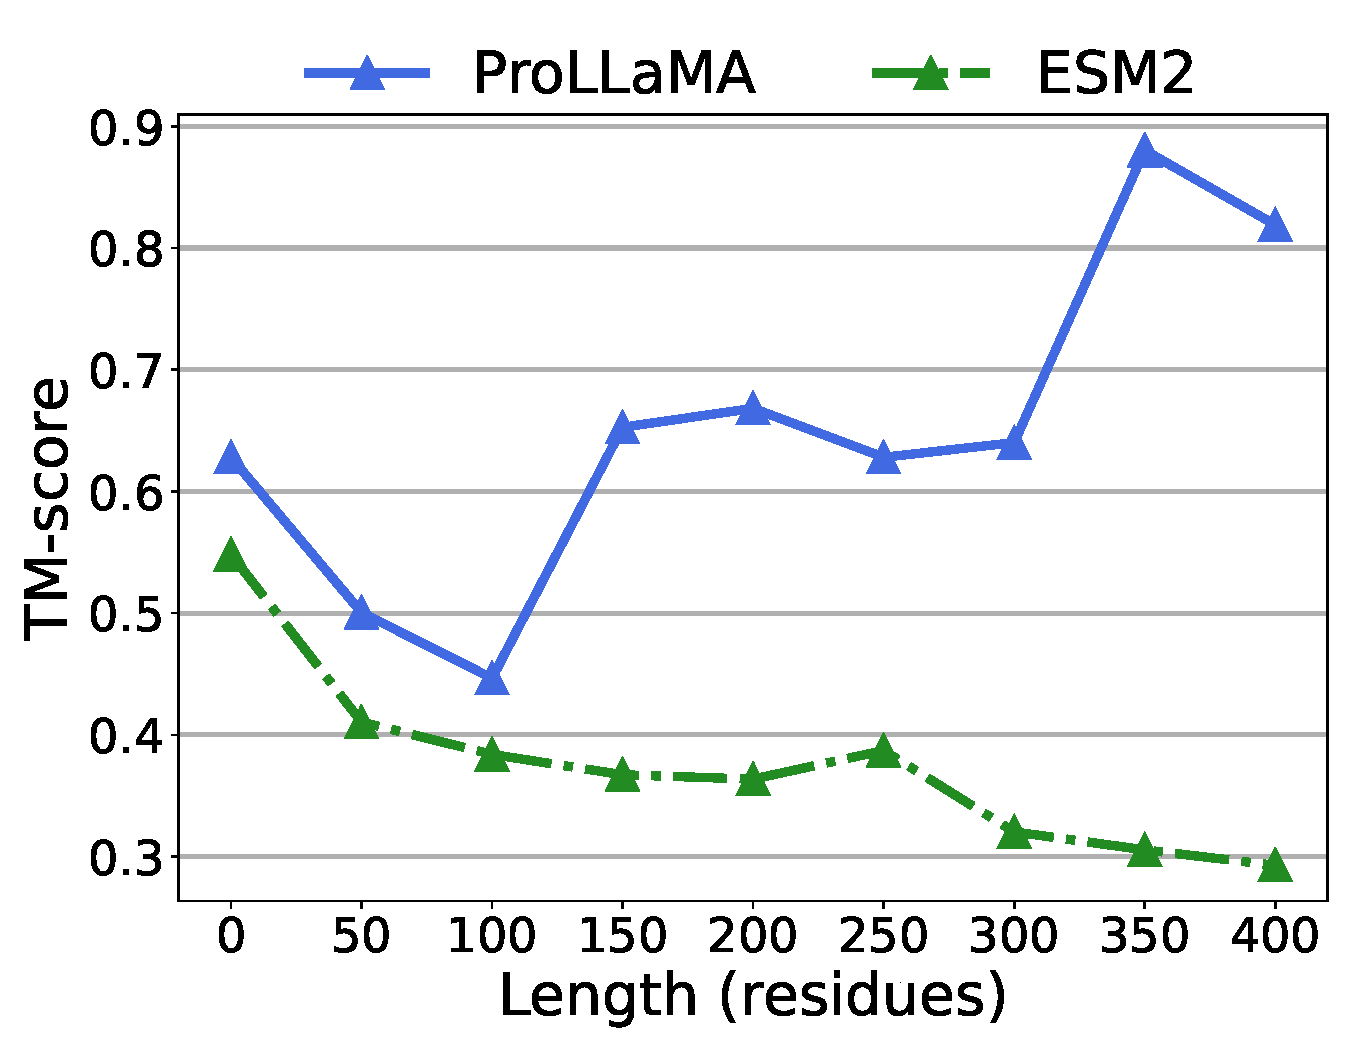
\includegraphics[scale=0.23]{images/combined_length_alntmscore_zhexiantu.pdf}
	\end{column}
	\begin{column}{0.5\textwidth}
		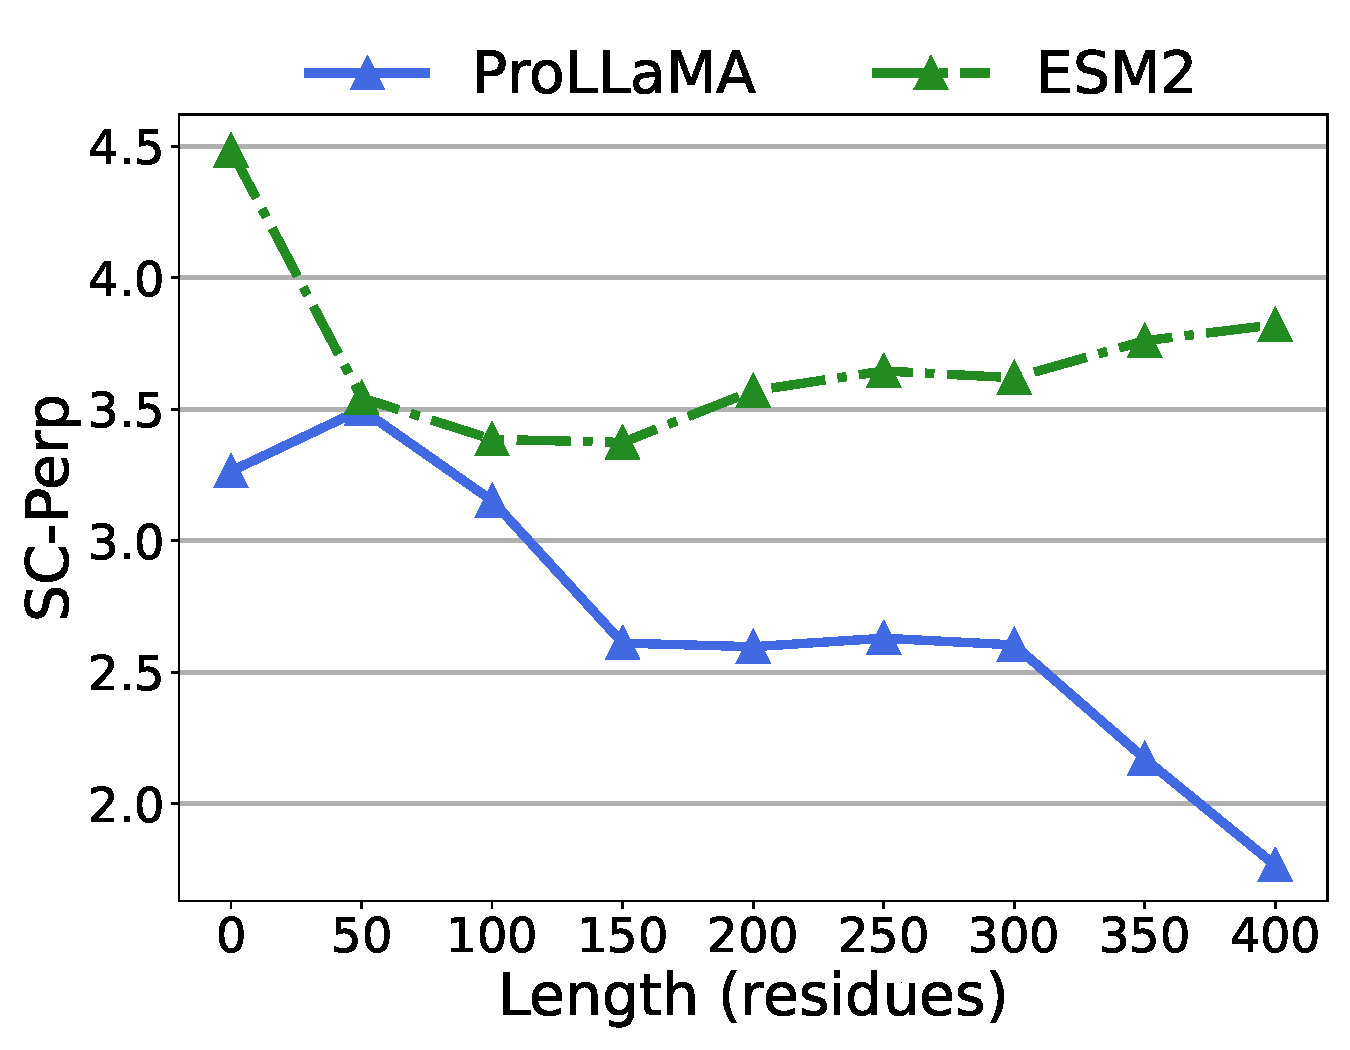
\includegraphics[scale=0.23]{images/combined_length_scperp_zhexiantu.pdf}
		\begin{itemize}
			\item ProLLaMA can capture long-range dependencies between amino acids.
		\end{itemize}
	\end{column}
\end{columns}
%\end{center}
\vspace{-2em}\credit{Image}{lv2024prollama}
\end{frame}